
\section*{Problem 1: Predicting Air Out Probability of Batted Balls}
\label{sec:p1}

Text here

\subsection{Data}
\label{subsec:data}

Notes:
\begin{enumerate}
  \item include horz exit angle as a 2nd-degree polynomial to capture non-linearities. (intuitively: the probability of an airout goes to zero as the ball flies straight into foul territory) - reference histogram
  \item vertical exit angle and exit speed are more informative when combined. For instance, a ball hit at a relatively high exit angle but low exit speed is much more likely to be a fly out than a ball hit at the same exit angle but with a very high exit speed.
\end{enumerate}

\begin{figure}[htb]
  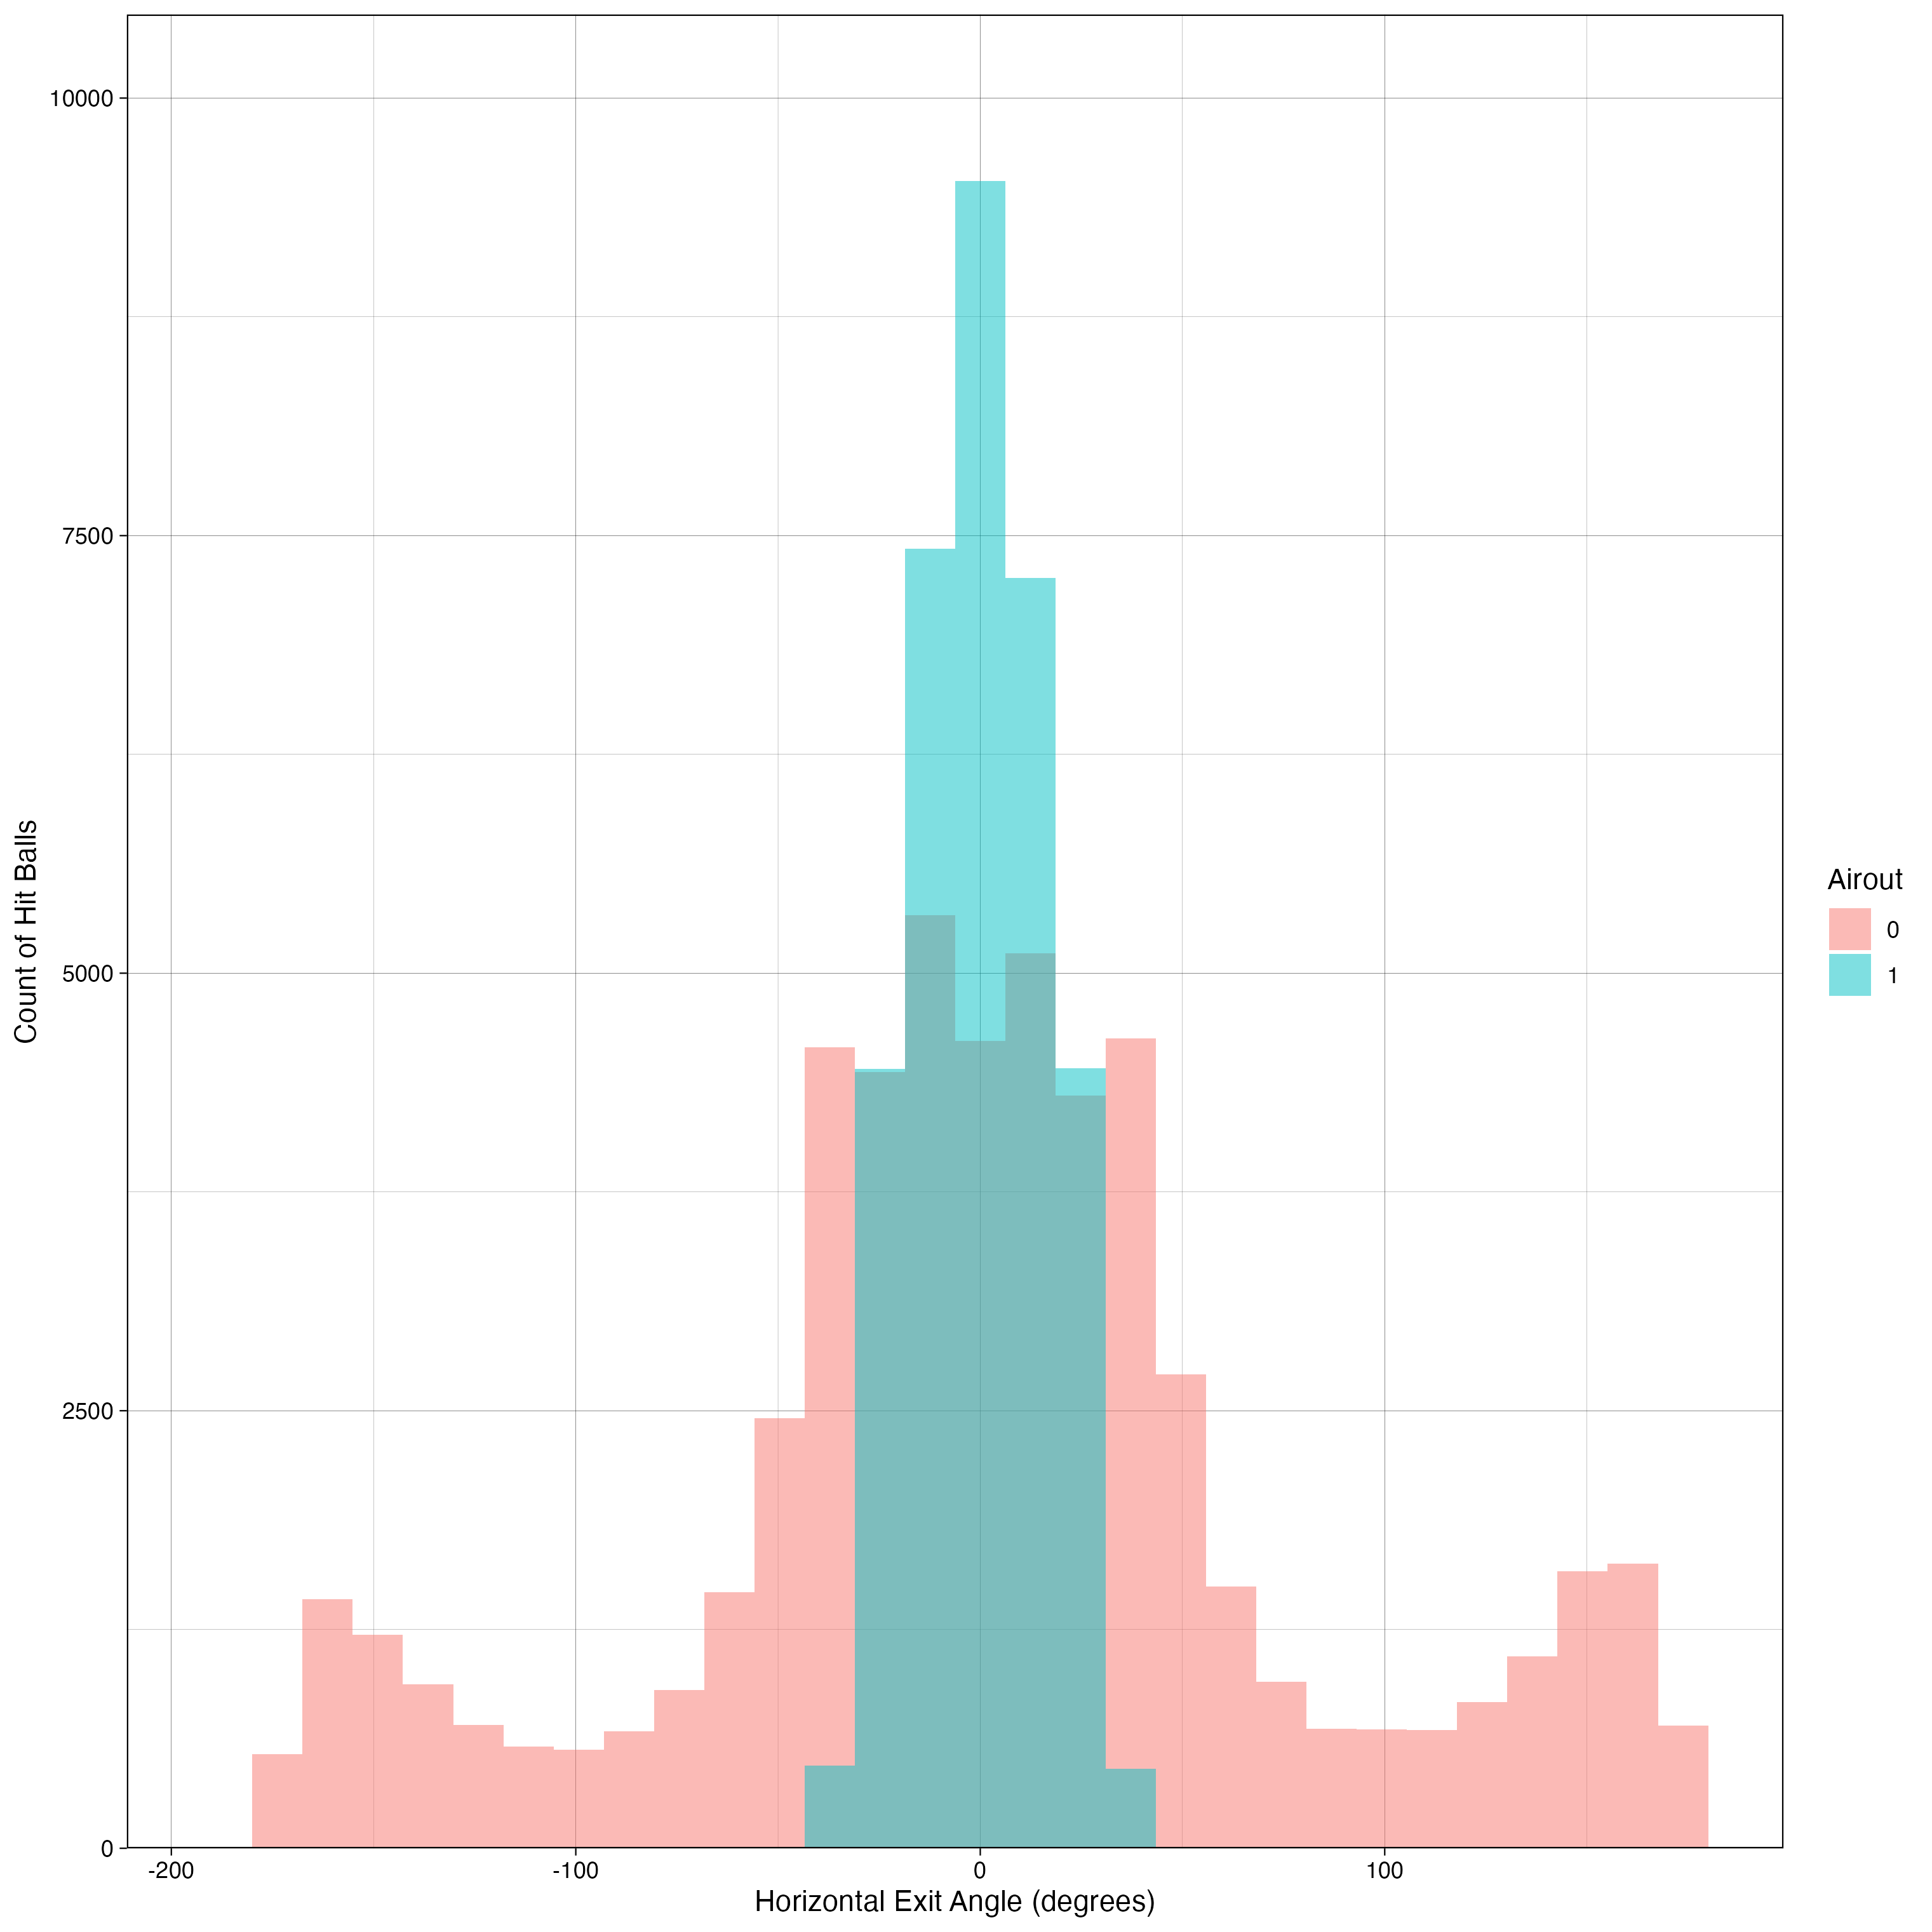
\includegraphics[width = 0.47\textwidth]{../../output/figs/horz_exit_angle_hist.png}
  \caption{Count of Hit Balls by Horizontal Exit Angle}
  \label{fig:hist}
\end{figure}

\begin{figure}[htb]
  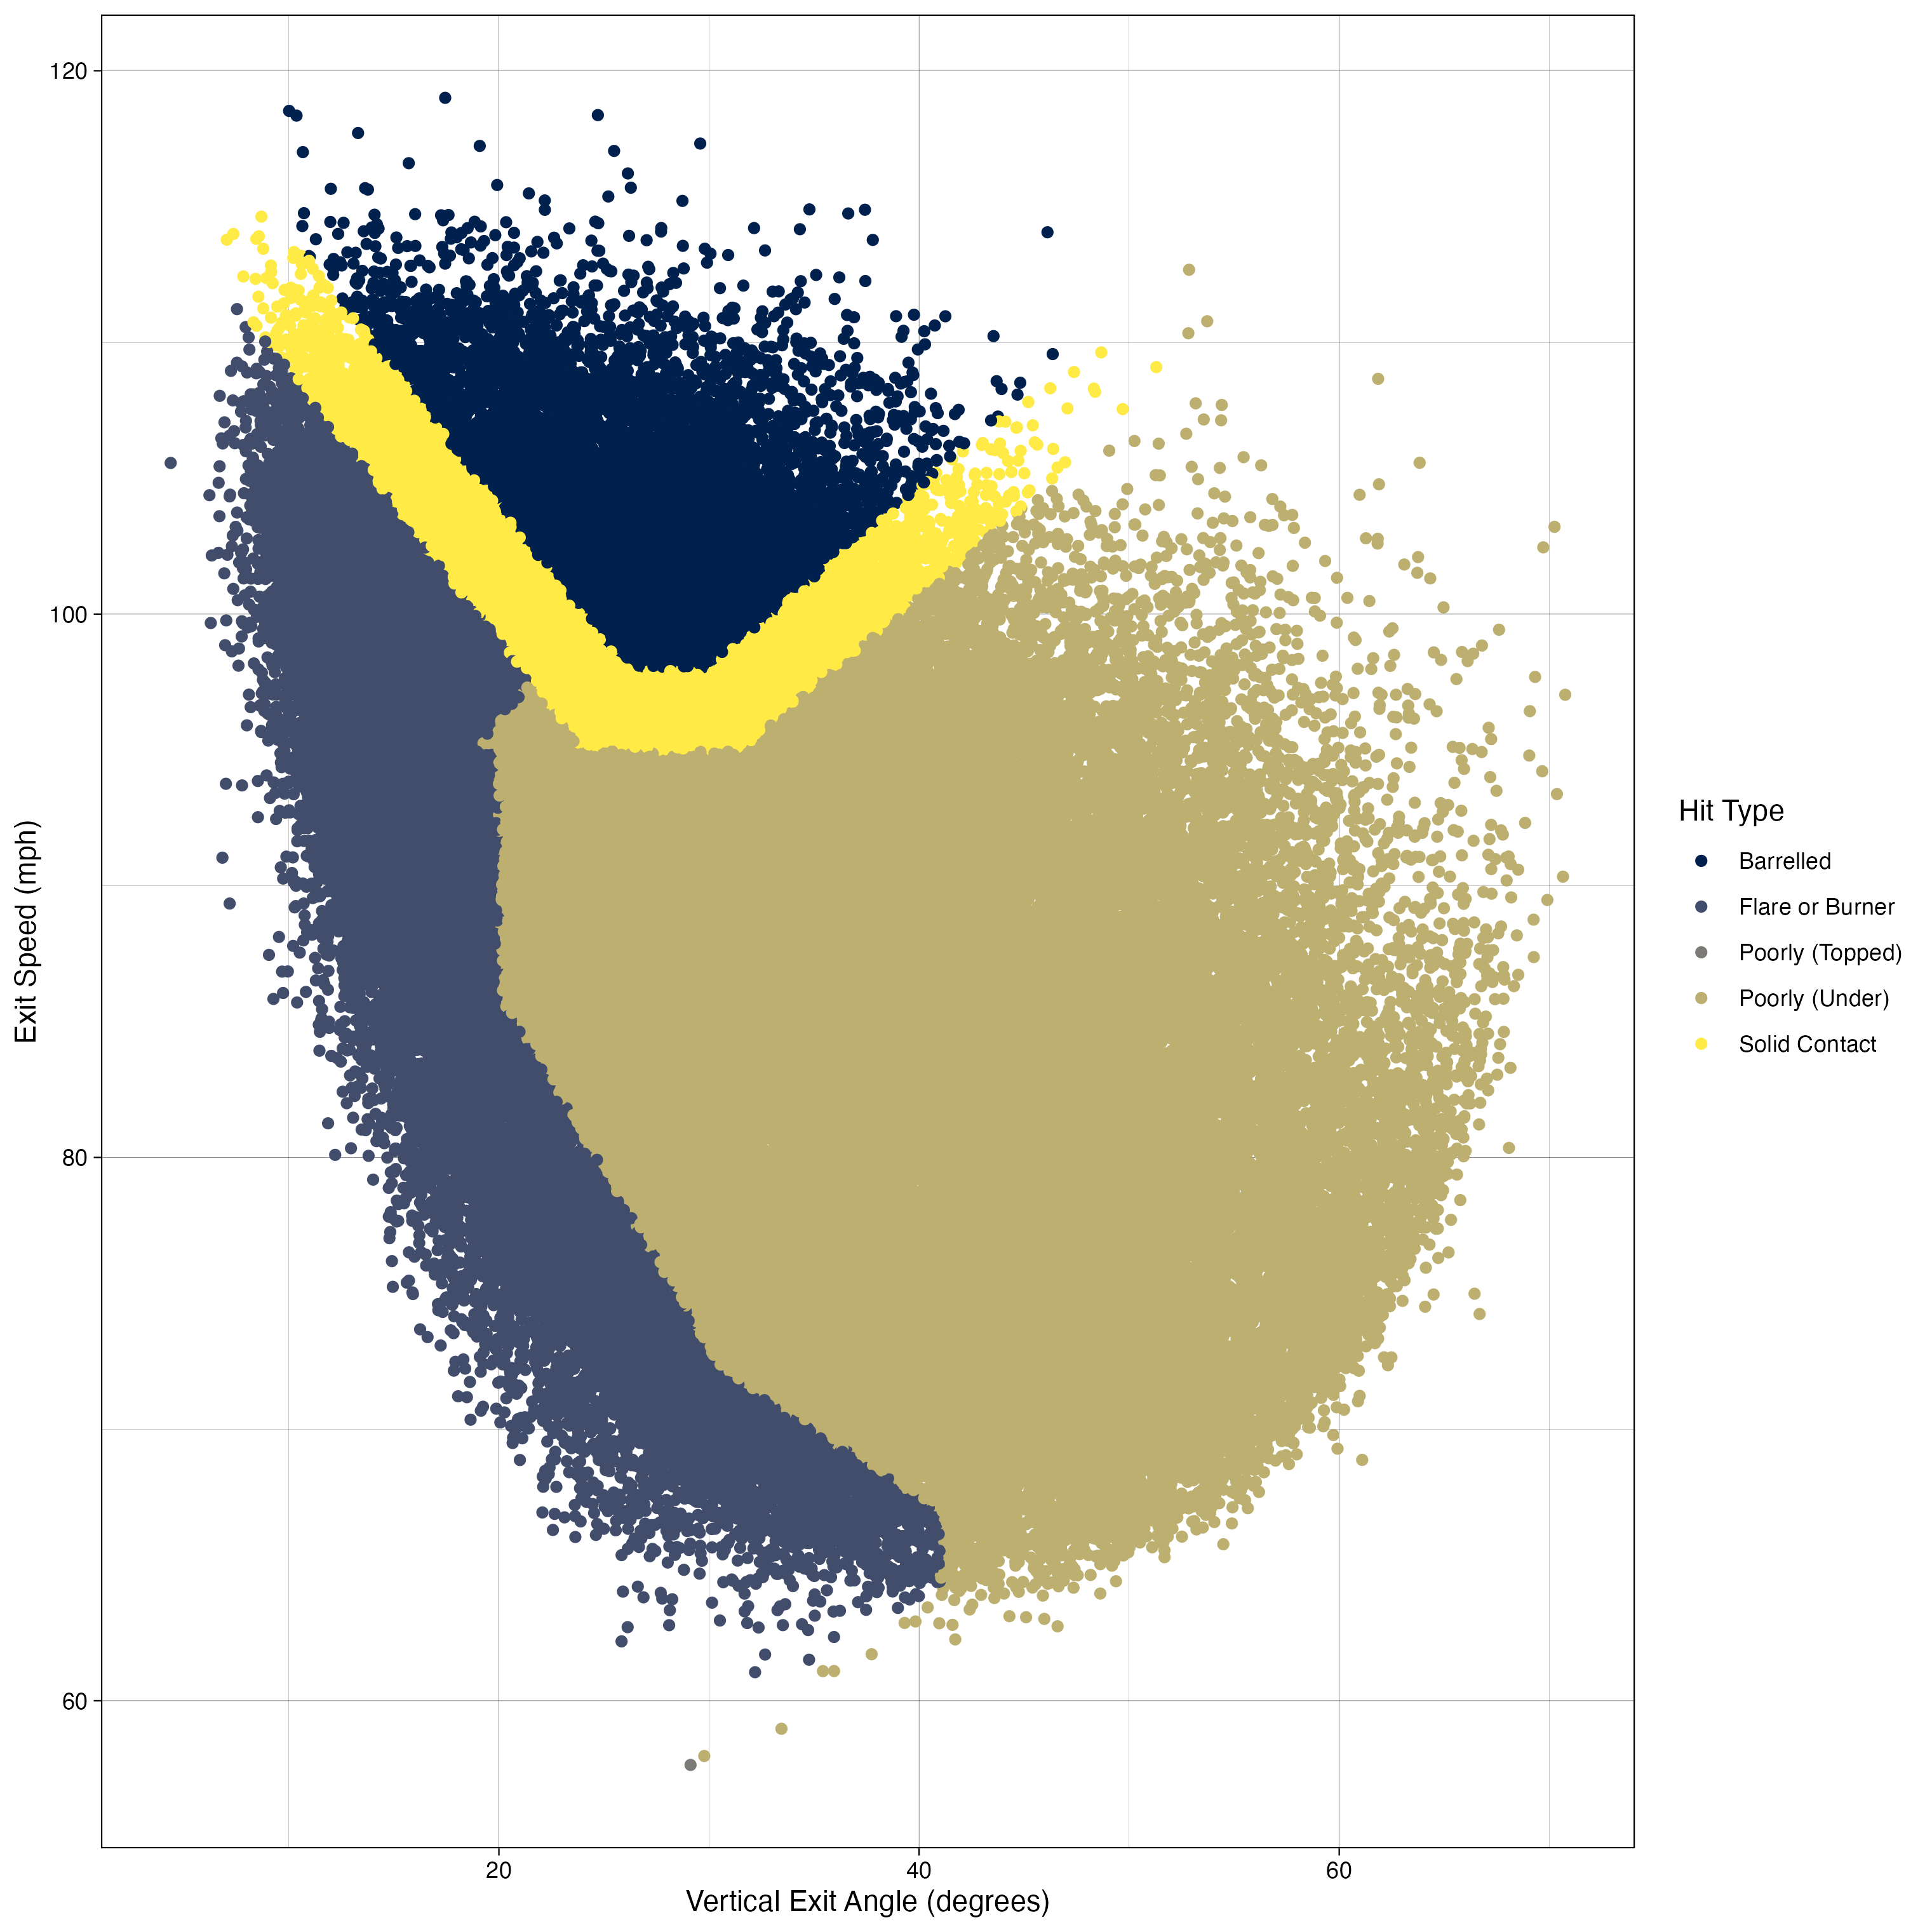
\includegraphics[width = 0.47\textwidth]{../../output/figs/barrelled.png}
  \caption{Hit Type by Exit Speed and Vertical Exit Angle}
  \label{fig:barrelled}
\end{figure}

\subsection{Modeling}
\label{subsec:model}

Notes here

\subsection{Results}
\label{subsec:results}

Notes here


